% Provenance (never printed): see sources/outline_sources.md (Year 3: gravity, magnetic,
% seismic, resistivity and ground-penetrating-radar surveys; data processing and
% uncertainty; a mapping project).
% Brief: sources/book5/BRIEFS.md, ch. 31. Curves from figdata/bachelor-3/gravity_granite.py
% (prism model of the Varden granite of figdata/shared/region.py), magnetic_dyke.py (2-D
% dyke; the Varden dolerite dyke of the Sync 3 ruling, buried below the unconformity),
% resistivity_sounding.py (Pekeris transform and image series) and gpr_radargram.py.
% Physical-property ranges and survey practice from the GPG open textbook (CC BY 4.0) and
% Keys (1990). Exercise and problem values in the Book 5 scratch calculator calc/ch31.py.
\chapter{Veld- en laboratoriummethoden III}\label{ch:b3:field-lab-methods-3}

Een geofysische ploeg brengt een week door in het dal van de Varden Hills, de
verzonnen streek waarvan de geologische kaart in het Boek~1 is getekend in
het hoofdstuk over geologische kaarten. De kaart toont een graniet dat aan de
zijkanten van het dal ontsluit, tussen de schisten, onder de zandsteen die op
beide rust. Waar het graniet onder de bedekking verdwijnt, hoe ver het
zich uitstrekt en hoe diep het reikt, heeft niemand ooit gezien. De ploeg draagt een
gravimeter, twee magnetometers, een kabel met elektroden en een radar op
een klein karretje. Geen van deze instrumenten ziet een gesteente: elk meet
een veld aan het oppervlak---de zwaartekracht, het magnetisch veld, een elektrische
potentiaal, de echo van een radiopuls---dat de gesteenten eronder verstoren.
Aan het eind van de week kan de ploeg het graniet tekenen dat zij nooit heeft gezien, zeggen
hoe diep het alluvium van de valleibodem is, en een magnetisch lichaam rapporteren
dat op geen enkele kaart stond.

Dit hoofdstuk volgt die week. Het behandelt elke methode om beurt, als een
meting met haar correcties en als een \omterm{def:b3:seismology-imaging:inverse}{voorwaarts probleem} met enkele
lichamen waarvan het veld exact kan worden berekend; daarna legt het uit hoe de
fouten van een onderzoek zich optellen en waarom één soort gegevens zelden een
model vastlegt; en het eindigt met het Varden-onderzoek, waar de methoden samen
worden gebracht.

\begin{recall}
De zwaartekrachtsanomalie, de vrije-luchtcorrectie en Bouguer-correctie en de
vrije-luchtanomalie en Bouguer-anomalie en de normale zwaartekracht staan in het Boek~1, in het hoofdstuk over isostasie
en zwaartekracht; de meetlus van een \omterm{def:b3:field-lab-methods-3:gravimeter}{relatieve gravimeter} wordt beschreven in
\cref{ch:b3:gravity-geodesy}. Het hoofdveld, de inclinatie, de
\omterm{thm:b3:palaeomagnetism:dipole}{dipoolformule} en de \omterm{def:b3:palaeomagnetism:igrf}{International Geomagnetic Reference Field} staan in
\cref{ch:b3:palaeomagnetism}. Soortelijke weerstand, de wet van Ohm, de relatieve
permittiviteit, elektromagnetische golven, magnetisatie en magnetische
susceptibiliteit staan in de natuurkundeboeken, en de wet van Gauss voor
de zwaartekracht ermee. Seismische refractieonderzoeken staan in
\cref{ch:b3:exploration-seismology}; voorwaartse en inverse problemen en
gewogen kleinste kwadraten in \cref{ch:b3:seismology-imaging}; porositeit in
de schoolboeken en \omterm{def:b3:facies-models:wireline}{boorgatlogs} in \cref{ch:b3:facies-models}. De
voortplanting van onzekerheden staat in de scheikunde- en wiskundeboeken.
\end{recall}

\section{Zwaartekrachtonderzoeken}\label{sec:b3:field-lab-methods-3:gravity}

De anomalieën waarnaar een zwaartekrachtonderzoek zoekt, zijn klein. De
zwaartekracht aan de evenaar bedraagt ongeveer \qty{978000}{\milli\gal}; grote
structuren veranderen haar met honderden milligal, een zoutkoepel met ongeveer
tien, een ertslichaam met ongeveer één, en de doelen van een geotechnisch
onderzoek met een paar honderdsten. Geofysici meten in
milligal, of in zwaartekrachtseenheden van \qty{0.1}{\milli\gal}; een bruikbaar
onderzoek moet verschillen van één deel op honderd miljoen van~$g$ onderscheiden.
% ledger: gpg:grav-units, gpg:grav-sizes

\begin{definition}[Relatieve gravimeter; instrumentele drift]\label{def:b3:field-lab-methods-3:gravimeter}
Een \emph{relatieve gravimeter}\index{relatieve gravimeter} is een instrument
dat verschillen in zwaartekracht tussen stations meet: een massa aan een veer,
op een nulpositie gehouden door een tweede, instelbare kracht waarvan de
wijzerstand, vermenigvuldigd met een ijkconstante, de zwaartekracht geeft in
milligal tot op een onbekende constante. Zijn \emph{instrumentele
drift}\index{instrumentele drift} is de langzame verandering van zijn aflezing op
een vast station, veroorzaakt door het kruipen van de veer, temperatuur en
schokken; hij wordt gemeten door na een paar uur opnieuw een reeds gelezen
station af te lezen, het \emph{basisstation}.
\end{definition}
% ledger: gpg:gravimeter, gpg:grav-survey

Een veldgravimeter bestrijkt een bereik van enkele tienduizenden milligal en
leest, op zijn best, af tot ongeveer \qty{0.01}{\milli\gal}; het bereik moet na
transport opnieuw worden ingesteld. Bij die precisie weegt de hoogte van elk
station even zwaar als de aflezing zelf: \qty{3.3}{cm} hoogtefout
bederft \qty{0.01}{\milli\gal}, dus de posities worden gemeten met
satellietontvangers of met een waterpas tot op de centimeter. Het basisstation
wordt om de paar uur opnieuw bezocht. De vaste-aardetij, die
\qty{0.3}{\milli\gal} kan bereiken, verandert over die uren zo langzaam dat hij
met de drift kan worden verwijderd.
% ledger: gpg:gravimeter, gpg:grav-survey, gpg:grav-sizes

\begin{method}[Een zwaartekrachtlus reduceren]\label{met:b3:field-lab-methods-3:loop}
Een lus begint en eindigt bij een basisstation, afgelezen op de tijdstippen $t_0$ en $t_1$.
\begin{enumerate}
  \item Bereken de driftsnelheid $(r_1 - r_0)/(t_1 - t_0)$ uit de twee
        basisaflezingen; zij bevat het getij.
  \item Trek van elke aflezing de drift af die sinds $t_0$ is opgelopen,
        $r - (t - t_0)(r_1 - r_0)/(t_1 - t_0)$, en trek de aflezing van het
        basisstation af: dit is de zwaartekracht ten opzichte van het basisstation.
  \item Corrigeer voor de hoogte $\Delta h$ van het station boven het basisstation:
        tel de vrije-luchtcorrectie $\qty{0.3086}{\milli\gal.m^{-1}}
        \times\Delta h$ op en trek de Bouguer-correctie
        $\qty{0.1119}{\milli\gal.m^{-1}}\times\Delta h$ af (dichtheid
        \qty{2670}{kg.m^{-3}}), dat wil zeggen, tel $0.1967\,\Delta h$ op.
  \item Voor een station op een afstand $\Delta y$ noordelijk van het basisstation, trek
        de verandering van de normale zwaartekracht af, $\qty{0.811}{\milli\gal.km^{-1}}
        \times\sin 2\varphi\times\Delta y$.
  \item Tel de \omterm{def:b3:field-lab-methods-3:terrain}{terreincorrectie} van elk station op.
\end{enumerate}
De uitkomst is de Bouguer-anomalie ten opzichte van het basisstation. Door het
basisstation te koppelen aan een station met bekende absolute zwaartekracht krijgt men de anomalie zelf.
\end{method}
% ledger: gpg:grav-survey, gpg:terrain

De Bouguer-correctie behandelt het terrein tussen het station en het
referentieniveau als een vlakke plaat. In echt reliëf is dit tweemaal fout:
een heuvel die boven het station uitsteekt trekt naar boven en verlaagt de
aflezing, en een vallei die onder het station daalt, wordt in de plaat meegerekend als
gesteente dat er niet is.

\begin{definition}[Terreincorrectie]\label{def:b3:field-lab-methods-3:terrain}
De \emph{terreincorrectie}\index{terreincorrectie} van een
zwaartekrachtstation is de aantrekking die de afwijkingen van het reliëf ten opzichte van de
Bouguer-plaat op het station uitoefenen: de heuvels boven het niveau van het station en
de dalen eronder, geteld met de dichtheid van de plaat. Beide verlagen
de gemeten zwaartekracht ten opzichte van de plaat, daarom wordt de
correctie altijd opgeteld.
\end{definition}

Zij werd met de hand berekend, met een Hammer-grafiek en tabellen, zone voor zone
vanaf het station naar buiten; tegenwoordig wordt zij berekend uit een digitaal
hoogtemodel. Ver van steil reliëf overschrijdt zij zelden \qty{1}{\milli\gal},
maar de zones dicht bij het station zijn moeilijk goed te krijgen, en de
correctie wordt zelden nauwkeuriger dan \qty{0.2}{\milli\gal} bekend.
% ledger: gpg:terrain, gpg:grav-sizes

\subsection{Anomalieën van eenvoudige lichamen}

Het \omterm{def:b3:seismology-imaging:inverse}{voorwaarts probleem} van de zwaartekracht is een som: elk element van een lichaam
met dichtheidscontrast $\Delta\rho$ trekt het station aan volgens de wet van Newton, en
een meting meet de verticale component van de som. Enkele lichamen geven
het in gesloten vorm.

\begin{theorem}[Bol en horizontale cilinder]\label{thm:b3:field-lab-methods-3:sphere}
Op een horizontale afstand $x$ van het punt boven het middelpunt van een
begraven bol met overmassa $\Delta m$, waarvan het middelpunt op diepte $z$ ligt, geeft de
anomalie:
\[
\Delta g(x) = \frac{G\,\Delta m\,z}{(x^2 + z^2)^{3/2}} ,
\]
en de anomalie zakt tot de helft van haar piek bij $x_{1/2} = z\sqrt{2^{2/3} - 1}$,
zodat $z = 1.305\,x_{1/2}$. Een lange horizontale cilinder met overmassa
$\lambda$ per eenheid van lengte, met zijn as op diepte $z$, geeft dwars op
de strekking
\[
\Delta g(x) = \frac{2G\lambda z}{x^2 + z^2} ,
\]
en $z = x_{1/2}$.
\end{theorem}

\begin{proof}
Buiten een bol waarvan de dichtheid alleen van de afstand tot zijn
middelpunt afhangt, is de aantrekking gelijk aan die van zijn massa in het middelpunt (de
schilstelling, een gevolg van de stelling van Gauss). De grootte op het
station is $G\Delta m/(x^2 + z^2)$, en de verticale component bevat
de factor $z/\sqrt{x^2 + z^2}$. Invullen van $\Delta g(x_{1/2}) =
\Delta g(0)/2$ levert $(1 + x_{1/2}^2/z^2)^{3/2} = 2$, vandaar de regel. Voor
de cilinder geeft de stelling van Gauss op een coaxiale cilinder met straal $r$
een veld $2G\lambda/r$, en de verticale component $2G\lambda z/r^2$;
de helft van de piek wordt bereikt als $x^2 + z^2 = 2z^2$.
\end{proof}
% ledger: gpg:half-width

Een lichaam dat geen bol is, heeft toch een halve breedte, en de regel geeft dan
de diepte van een equivalente bol, niet van het lichaam. De regel is
een eerste schatting, gemaakt voordat er een model is aangepast.

\begin{proposition}[Verticale cilinder op zijn as]\label{prop:b3:field-lab-methods-3:vcyl}
Een verticale cilinder met straal $a$ en dichtheidscontrast $\Delta\rho$,
waarvan de bovenkant en onderkant op diepten $z_1 < z_2$ onder het station liggen,
geeft op zijn as
\[
\Delta g = 2\pi G\Delta\rho\left[(z_2 - z_1) + \sqrt{z_1^2 + a^2}
           - \sqrt{z_2^2 + a^2}\right] .
\]
Voor $a \to \infty$ is het de Bouguer-plaat $2\pi G\Delta\rho(z_2 - z_1)$;
voor een cilinder van het oppervlak tot grote diepte gaat hij naar
$2\pi G\Delta\rho\,a$.
\end{proposition}

\begin{proof}
Een schijf met straal $a$ en dikte $\mathrm{d}z$ op diepte $z$ trekt
een punt op zijn as aan met $2\pi G\Delta\rho\,\mathrm{d}z\,(1 -
z/\sqrt{z^2 + a^2})$, de aantrekking van een ring, geïntegreerd over de
straal. Integreren van $z_1$ tot $z_2$ levert de term tussen haakjes. Als $a \to
\infty$ bij vaste diepten, $\sqrt{z_1^2 + a^2} - \sqrt{z_2^2 + a^2} =
(z_1^2 - z_2^2)/(\sqrt{z_1^2 + a^2} + \sqrt{z_2^2 + a^2}) \to 0$; als
$z_1 = 0$ en $z_2 \to \infty$, $z_2 - \sqrt{z_2^2 + a^2} \to 0$ en
de term tussen haakjes naar $a$.
\end{proof}

\begin{proposition}[Overmassa uit een zwaartekrachtkaart]\label{prop:b3:field-lab-methods-3:gauss}
Ongeacht de vorm van een lichaam dat volledig onder een horizontaal
vlak ligt, is de overmassa
\[
\Delta m = \frac{1}{2\pi G}\iint \Delta g\,\mathrm{d}A ,
\]
waarbij de integraal het hele vlak bestrijkt.
\end{proposition}

\begin{proof}
Voor een puntmassa $m$ op diepte $z$, met $r$ de horizontale afstand,
$\iint \Delta g\,\mathrm{d}A = \int_0^\infty
Gmz\,(r^2 + z^2)^{-3/2}\,2\pi r\,\mathrm{d}r = 2\pi Gm$: de helft van de flux
$4\pi Gm$ van de stelling van Gauss gaat door het vlak. Een lichaam is een som van
puntmassa's, en de integraal is lineair.
\end{proof}

De stelling geeft de massa, nooit de vorm; en een kaart bestrijkt slechts een deel
van het vlak, terwijl de anomalie van een diep lichaam langzaam afneemt, zodat de
massa die uit een kaart volgt, te klein is tenzij de randen door een
model worden verlengd.

\begin{omfigure}
\begin{tikzpicture}
\begin{axis}[axis equal image, xmin=1.5, xmax=5.5, ymin=2.6, ymax=5.7, width=0.86\linewidth,
  tick label style={font=\scriptsize}, xlabel={oost (km)}, ylabel={noord (km)},
  label style={font=\small}, unbounded coords=jump]
% geology of the region (figdata/shared/region.py), faded
\addplot[lith schist, draw=black!50, line width=0.2pt, even odd rule, opacity=0.45] table {figdata/out/shared-region-unit-schist.dat};
\addplot[lith granite, draw=black!50, line width=0.2pt, even odd rule, opacity=0.45] table {figdata/out/shared-region-unit-granite.dat};
\addplot[om lith={icsTriassic!35}{om sand}, draw=black!50, line width=0.2pt, even odd rule, opacity=0.45] table {figdata/out/shared-region-unit-sandstone.dat};
\addplot[om lith={icsJurassic!40}{om limestone}, draw=black!50, line width=0.2pt, even odd rule, opacity=0.45] table {figdata/out/shared-region-unit-limestone.dat};
\addplot[om lith={icsJurassic!15}{om shale}, draw=black!50, line width=0.2pt, even odd rule, opacity=0.45] table {figdata/out/shared-region-unit-shale.dat};
\addplot[lith alluvium, draw=black!50, line width=0.2pt, even odd rule, opacity=0.45] table {figdata/out/shared-region-unit-alluvium.dat};
\addplot[river] table {figdata/out/shared-region-river.dat};
% the survey (figdata/bachelor-3/gravity_granite.py, magnetic_dyke.py)
\addplot[only marks, mark=*, mark size=0.7pt, black!70] table[x=x_km, y=y_km] {figdata/out/bachelor-3-gravity_granite-stations.dat};
\addplot[omDef, very thick] table[x=x_km, y=y_km] {figdata/out/bachelor-3-gravity_granite-contours.dat};
\addplot[omThm, thick] coordinates {(1.5,4.15) (5.5,4.15)};
\addplot[omMeth, line width=2.2pt, opacity=0.8] coordinates {(1.7,4.15) (2.7,4.15)};
\addplot[omProp, dashed, thick] coordinates {(2.2,2.6) (2.2,5.7)};
\addplot[only marks, mark=star, mark size=3.5pt, omMeth!70!black, thick] coordinates {(3.5,4.0)};
\node[font=\scriptsize, fill=white, fill opacity=0.85, text opacity=1, inner sep=1pt] at (axis cs:3.5,5.12) {$-0.5$};
\node[font=\scriptsize, fill=white, fill opacity=0.85, text opacity=1, inner sep=1pt] at (axis cs:3.5,4.84) {$-1$};
\node[font=\scriptsize, fill=white, fill opacity=0.85, text opacity=1, inner sep=1pt] at (axis cs:3.5,4.58) {$-2$};
\node[font=\scriptsize, anchor=south west, fill=white, fill opacity=0.85, text opacity=1, inner sep=1pt] at (axis cs:1.55,4.17) {zwaartekrachtprofiel};
\node[font=\scriptsize, anchor=north, fill=white, fill opacity=0.85, text opacity=1, inner sep=1pt] at (axis cs:2.2,4.08) {magnetische lijn};
\node[font=\scriptsize, anchor=north west, text=omProp!80!black, fill=white, fill opacity=0.85, text opacity=1, inner sep=1pt] at (axis cs:2.24,5.6) {begraven gang};
\node[font=\scriptsize, anchor=north, fill=white, fill opacity=0.85, text opacity=1, inner sep=1pt] at (axis cs:3.5,3.92) {peiling};
\pic at (axis cs:5.15,5.3) {northarrow};
\end{axis}
\end{tikzpicture}

\par\smallskip{\small De Varden-meting over de geologische kaart van het gebied
(vervaagd: schist grijs, graniet roze, zandsteen, kalksteen en schalie van de
bedekking, alluvium langs de rivier). Zwarte stippen: de zwaartekrachtstations,
\qty{200}{m} uit elkaar; blauw: de Bouguer-anomalie van het granietmodel,
met contourlijnen elke \qty{0.5}{\milli\gal}; rood: het zwaartekrachtprofiel;
groen: de magnetische lijn en de elektrische peiling (ster) op de
bodem van de vallei; oranje gestreept: de doleriet-gang die de magnetische meting vindt,
begraven onder de bedekking.}\label{fig:b3:field-lab-methods-3:survey}
\end{omfigure}
% ledger: gpg:densities

\subsection{Het Varden-graniet}

Het model van de geologen voor het graniet is een elliptisch lichaam onder de
discordantie, \qty{760}{m} breed in oost--west-richting en \qty{1120}{m} in
noord--zuid-richting waar het de bedekking raakt, en het wordt naar beneden
breder; aan de dalflanken komt het aan het oppervlak. Graniet is lichter dan
schist: de gepubliceerde dichtheidsbereiken zijn \numrange{2.50}{2.81} en
\qtyrange{2.39}{2.80}{g.cm^{-3}}. Het model van de meting neemt
\qty{2620}{kg.m^{-3}} voor het graniet en \qty{2750}{kg.m^{-3}} voor de
schist, een contrast van \qty{-130}{kg.m^{-3}}, en stopt het graniet op
\qty{1500}{m} onder zeeniveau, een aanname omdat niets de onderkant toont.
Na opdeling in \num{5533} rechte prisma's waarvan de aantrekkingen een
gesloten vorm hebben, geeft het model de anomalie van de kaart hierboven: een
gesloten minimum van \qty{-2.29}{\milli\gal} boven het midden van het graniet,
met contouren die noord--zuid langgerekt zijn, net als het lichaam.
% ledger: gpg:densities

\begin{omfigure}
\begin{tikzpicture}
\begin{axis}[width=0.8\linewidth, height=0.42\linewidth, xmin=1.5, xmax=5.5, ymin=-2.6, ymax=0.2,
  xlabel={oost (km)}, ylabel={$\Delta g$ (\unit{\milli\gal})},
  tick label style={font=\scriptsize}, label style={font=\small},
  legend style={font=\scriptsize, at={(0.02,0.04)}, anchor=south west}]
% computed in figdata/bachelor-3/gravity_granite.py
\addplot[omDef, very thick] table[x=x_km, y=dg_mGal] {figdata/out/bachelor-3-gravity_granite-profile.dat};
\addlegendentry{granietmodel}
\addplot[omThm, densely dashed, thick] table[x=x_km, y=sphere] {figdata/out/bachelor-3-gravity_granite-profile.dat};
\addlegendentry{bol van de halfbreedteregel}
\addplot[omMeth, densely dotted, thick] table[x=x_km, y=cyl] {figdata/out/bachelor-3-gravity_granite-profile.dat};
\addlegendentry{verticale cilinder}
\addplot[black!40, forget plot] coordinates {(1.5,0) (5.5,0)};
\addplot[black!50, densely dotted, forget plot] coordinates {(1.5,-1.1464) (5.5,-1.1464)};
\node[font=\scriptsize, black!60, anchor=south east] at (axis cs:5.45,-1.14) {halve piek};
\end{axis}
\end{tikzpicture}

\par\smallskip{\small De anomalie langs het zwaartekrachtprofiel (blauw), de
bol waarvan diepte en massa de halfbreedteregel geeft (rood gestreept), en
een verticale cilinder met hetzelfde oppervlak als het graniet op de
discordantie, van het maaiveld tot de onderkant van het model (groen
gestippeld). De bol komt door constructie overeen met de piek en de
halfbreedte, maar niet met de flanken; de cilinder, die het breder worden
van het lichaam negeert, schiet tekort in het midden.}\label{fig:b3:field-lab-methods-3:profile}
\end{omfigure}
% ledger: gpg:half-width

\section{Magnetische metingen}\label{sec:b3:field-lab-methods-3:magnetics}

Het hoofdveld van de Aarde is ongeveer \qty{25000}{nT} aan de magnetische evenaar
en ongeveer \qty{70000}{nT} nabij de magnetische polen. Gesteenten die magnetiet
bevatten, voegen daar een eigen veld aan toe, geïnduceerd door het hoofdveld
in verhouding tot hun susceptibiliteit, of remanent, meegenomen vanaf het
moment waarop ze zijn gevormd. Een felsisch stollingsgesteente heeft een
susceptibiliteit onder ongeveer \num{2e-3}, een mafisch gesteente van ongeveer
\num{2e-3} tot \num{0.4}; op dezelfde schaal geeft één procent magnetiet per volume ongeveer \num{0.03}.
% ledger: gpg:mag-field, gpg:susceptibility

\begin{definition}[Totaalveldanomalie; dagelijkse correctie; reductie naar de pool]\label{def:b3:field-lab-methods-3:magnetic}
Laat $\mathbf{F}$ het hoofdveld op de meting zijn en $\Delta\mathbf{B}$
het veld van de gemagnetiseerde gesteenten.
\begin{itemize}
  \item De \emph{totaalveldanomalie}\index{totaalveldanomalie} is de gemeten
        intensiteit minus die van het hoofdveld, $\Delta T =
        |\mathbf{F} + \Delta\mathbf{B}| - |\mathbf{F}|$; wanneer
        $|\Delta\mathbf{B}| \ll |\mathbf{F}|$ is het de projectie
        $\Delta\mathbf{B}\cdot\mathbf{F}/|\mathbf{F}|$.
  \item De \emph{dagelijkse correctie}\index{dagelijkse correctie} verwijdert
        de variaties van het veld in de tijd: een magnetometer op een vast
        basisstation registreert het veld gedurende de hele meting, en elke
        aflezing $T(t)$ van het bewegende instrument wordt vervangen door $T(t) -
        T_\mathrm{base}(t)$.
  \item De \emph{reductie naar de pool}\index{reductie naar de pool}
        berekent uit de gemeten anomalie de anomalie die dezelfde gesteenten
        zouden geven als het hoofdveld verticaal was, zoals op een magnetische
        pool; de anomalie ligt dan recht boven de bron.
\end{itemize}
\end{definition}
% ledger: gpg:mag-survey, gpg:mag-processing

De variaties in de tijd komen van stromen in de ionosfeer, ongeveer
\qty{110}{km} hoog. Op één dag bedragen ze gewoonlijk ongeveer
\qtyrange{20}{50}{nT}, evenveel als de anomalie van een klein doel; een
magnetische storm kan het veld met duizenden nanotesla veranderen. Het
basisstation meet de variatie, in de veronderstelling dat zij over de hele
meting gelijk is. Het hoofdveld zelf, of het veld van structuren die groter
zijn dan de meting, wordt verwijderd met de IGRF, een constante of een
aangepaste trend.
% ledger: gpg:mag-field, gpg:mag-processing

Een protonprecessiemagnetometer meet de frequentie waarmee de protonspins
in het veld precesseren, die evenredig is met het veld; hij leest af tot
\qty{1}{nT} en heeft meer dan een seconde nodig per aflezing. Een optisch
gepompte cesiummagnetometer is tien tot honderd keer gevoeliger en leest af
tot \qty{0.01}{nT}. De stations moeten dicht genoeg bij elkaar liggen om
minstens ongeveer drie aflezingen over de halfbreedte van de smalste gezochte
anomalie te krijgen, en hoe ondieper de bron, hoe dichter ze bij elkaar moeten liggen.
moet zijn.
% ledger: gpg:mag-survey

\begin{proposition}[Anomalie van een dunne gang]\label{prop:b3:field-lab-methods-3:dyke}
Een verticale gang met dikte $t$ en susceptibiliteit $\kappa$, lopend
langs de magnetische meridiaan, met de bovenkant op diepte $z$ en zich ver
naar beneden uitstrekkend, gemagnetiseerd door inductie in een hoofdveld $F$ met inclinatie $I$,
geeft dwars op zijn strekking, als $t \ll z$,
\[
\Delta T(x) = \frac{\kappa F t\sin^2 I}{2\pi}\,\frac{z}{x^2 + z^2} ,
\]
een symmetrische anomalie die tot de helft van haar piek daalt bij $x = \pm z$: de
diepte tot de bovenkant van de gang is de helft van de volle breedte van de anomalie op
de helft van haar piek.
\end{proposition}

\begin{proof}
De gang is tweedimensionaal en het hoofdveld ligt in het verticale
De magnetisatie $\mathbf{M} = \kappa\mathbf{F}/\mu_0$
heeft een component langs de strekking, waarvan de polen aan de uiteinden van de
gang ver weg liggen en die geen veld geeft; en een verticale component $M
\sin I$, die op het bovenvlak van de gang een magnetische lading van
$-Mt\sin I$ per lengte-eenheid (met $\mathbf{M}\cdot\mathbf{n}$ als de
ladingsdichtheid, $\mathbf{n}$ de uitwaartse normaal), waarbij het ondervlak
ver weg ligt. Een lijnlading $q$ per lengte-eenheid geeft, volgens de stelling van Gauss
in twee dimensies, een veld $q/(2\pi r)$ langs de straal. Op een
station op $(x, 0)$ boven een top op $(0, z)$ is de neerwaartse component
$Mt\sin I\,z/(2\pi(x^2 + z^2))$, en de horizontale component is
dwars op de strekking, loodrecht op $\mathbf{F}$. Vermenigvuldigd met
$\mu_0$ en geprojecteerd op $\mathbf{F}$, waarvan de verticale component is
$\sin I$, levert $\Delta T$. De voorwaarde voor de halve piek is $x^2 + z^2 =
2z^2$.
\end{proof}

Wanneer de gang de meridiaan kruist, liggen de horizontale delen van de
magnetisatie en van het hoofdveld beide in het vlak van het
profiel, de zijvlakken dragen ladingen, en de anomalie wordt
asymmetrisch, met een dal aan de kant van de pool. De figuur hieronder
berekent haar exact voor een gang met eindige breedte, door de gesloten
velden van de vier geladen vlakken op te tellen. De \omterm{def:b3:field-lab-methods-3:magnetic}{reductie naar de pool} zet zo'n
anomalie weer om in de symmetrische van een verticaal veld.

\begin{omfigure}
\begin{tikzpicture}
\begin{groupplot}[group style={group size=2 by 1, horizontal sep=1.5cm},
  width=0.48\linewidth, height=0.42\linewidth,
  tick label style={font=\scriptsize}, label style={font=\small}, title style={font=\small}]
\nextgroupplot[xmin=-600, xmax=600, ymin=-6, ymax=28, xlabel={afstand (\unit{m})},
  ylabel={$\Delta T$ (\unit{nT})}, title={een gang bij twee inclinaties},
  scaled x ticks=false,
  legend style={font=\scriptsize, at={(0.98,0.98)}, anchor=north east}]
% computed in figdata/bachelor-3/magnetic_dyke.py
\addplot[omDef, very thick] table[x=x_m, y=dT_I90] {figdata/out/bachelor-3-magnetic_dyke-generic.dat};
\addlegendentry{$I = 90^\circ$}
\addplot[omThm, thick] table[x=x_m, y=dT_I60] {figdata/out/bachelor-3-magnetic_dyke-generic.dat};
\addlegendentry{$60^\circ$, O--W strekking}
\addplot[omMeth, densely dashed, thick] table[x=x_m, y=dT_I60ns] {figdata/out/bachelor-3-magnetic_dyke-generic.dat};
\addlegendentry{$60^\circ$, N--Z strekking}
\addplot[black!40, forget plot] coordinates {(-600,0) (600,0)};
\node[font=\scriptsize, black!60, anchor=south west] at (axis cs:-590,-5.6) {Z};
\node[font=\scriptsize, black!60, anchor=south east] at (axis cs:590,-5.6) {N};
\nextgroupplot[xmin=1.7, xmax=2.7, ymin=0, ymax=40, xlabel={oost (km)},
  ylabel={veld $- \qty{48000}{nT}$}, title={de Varden-lijn, zoals afgelezen},
  legend style={font=\scriptsize, at={(0.02,0.98)}, anchor=north west}]
\addplot[omDef, thick, mark=*, mark size=1.1pt] table[x=x_km, y expr=\thisrow{T_obs}-48000] {figdata/out/bachelor-3-magnetic_dyke-line.dat};
\addlegendentry{bewegend instrument}
\addplot[omThm, thick, densely dashed] table[x expr=1.7+\thisrow{t_min}/40, y expr=\thisrow{T_base}-48000] {figdata/out/bachelor-3-magnetic_dyke-base.dat};
\addlegendentry{basisstation}
\end{groupplot}
\end{tikzpicture}

\par\smallskip{\small Links: de \omterm{def:b3:field-lab-methods-3:magnetic}{totaalveldanomalie} van een verticale gang
\qty{20}{m} dik, met de bovenkant \qty{100}{m} diep, susceptibiliteit \num{0.01},
in een veld van \qty{50000}{nT}; op profielen over een O--W strekking
bij inclinaties van \ang{90} en \ang{60}, en over een N--Z
strekking bij \ang{60}. Rechts: de aflezingen langs de magnetische Varden-lijn,
een station om de \qty{50}{m} en elke twee minuten, van W naar O,
en het basisstation op dezelfde tijdstippen (uitgezet op de positie waar het
bewegende instrument dan was): de stijging van het veld overdag is de helft van de
grootte van de anomalie.}\label{fig:b3:field-lab-methods-3:magnetic}
\end{omfigure}
% ledger: gpg:mag-field, gpg:susceptibility

\section{Elektrische methoden}\label{sec:b3:field-lab-methods-3:electrical}

De soortelijke weerstand varieert over een breder bereik dan elke andere eigenschap van gesteenten:
onverweerde stollingsgesteenten en metamorfe gesteenten liggen tussen ongeveer
\num{1000} en \qty{100000}{\ohm\metre}, schalies tussen ongeveer
\num{3} en \num{30}, droog grind en zand tussen enkele honderden en
tienduizend; zoet water ligt tussen ongeveer \num{1.5} en
\qty{130}{\ohm\metre} en zout water onder één. Poriewater geleidt
beter dan de meeste gesteentevormende mineralen, door zijn ionen, zodat de stroom
vooral door de poriën loopt, en de porositeit, de verzadiging en
het zoutgehalte van het water bepalen de soortelijke weerstand van een gesteente.
% ledger: gpg:resistivity, gpg:conduction

\begin{theorem}[Puntbron op een homogene ondergrond]\label{thm:b3:field-lab-methods-3:point-source}
Een stroom $I$ die in een punt van het oppervlak van een homogene ondergrond
met soortelijke weerstand $\rho$ wordt ingebracht, geeft op afstand $r$ de potentiaal
\[
V(r) = \frac{\rho I}{2\pi r} .
\]
Met twee stroomelektroden A~($+I$) en B~($-I$) en twee
potentiaalelektroden M en N is het gemeten potentiaalverschil
\[
\Delta V_{MN} = \frac{\rho I}{2\pi}\left(\frac{1}{AM} - \frac{1}{BM}
               - \frac{1}{AN} + \frac{1}{BN}\right) .
\]
\end{theorem}

\begin{proof}
Uit symmetrie stroomt de stroom radiaal en doorkruist elke halve bol met
straal $r$, met oppervlak $2\pi r^2$, uniform: $j = I/(2\pi r^2)$. De wet van Ohm
geeft het veld $E = \rho j$, en $V(r) = \int_r^\infty E\,\mathrm{d}r'
= \rho I/(2\pi r)$, met $V = 0$ ver weg. De potentialen van de twee
elektroden tellen op.
\end{proof}

\begin{definition}[Schijnbare soortelijke weerstand; elektrodeopstelling; verticale elektrische peiling; elektrische weerstandstomografie]\label{def:b3:field-lab-methods-3:resistivity}
\leavevmode
\begin{itemize}
  \item De \emph{schijnbare soortelijke weerstand}\index{schijnbare soortelijke weerstand} van een
        vierelektrodemeting is $\rho_a = K\,\Delta V_{MN}/I$, met
        de geometrische factor $K = 2\pi/(1/AM - 1/BM - 1/AN + 1/BN)$: de
        soortelijke weerstand van de homogene grond die dezelfde
        meetwaarde zou geven.
  \item Een \emph{elektrodeopstelling}\index{elektrodeopstelling} is een voorschrift dat
        de vier elektroden plaatst: de \emph{Wenner}-opstelling plaatst ze
        op gelijke afstand, $a$ van elkaar, in de volgorde AMNB; de
        \emph{Schlumberger}-opstelling plaatst M en N, $2l$ van elkaar, in het
        midden van een veel langere AB, met halve lengte $s$; dipool--dipool-,
        pool--dipool- en pool--poolopstellingen scheiden het stroompaar
        van het potentiaalpaar of sturen één elektrode ver weg.
  \item Een \emph{verticale elektrische peiling}\index{verticale elektrische peiling}
        breidt een opstelling uit rond een vast middelpunt en zet
        $\rho_a$ uit tegen de elektrodeafstand op logaritmische schalen: hoe
        groter de afstand, hoe dieper de stroom doordringt.
  \item \emph{Elektrische weerstandstomografie}\index{elektrische weerstandstomografie}
        plaatst veel elektroden langs een lijn,
        meet veel vierelektrodecombinaties en inverteert ze
        samen tot een doorsnede van de soortelijke weerstand.
\end{itemize}
\end{definition}
% ledger: gpg:dc-survey

Voor de Wenner-opstelling is de factor $K = 2\pi a$; voor de Schlumberger-
opstelling $K = \pi(s^2 - l^2)/(2l)$, en $\rho_a \approx 2\pi s^2(-\mathrm{d}V/
\mathrm{d}r)/I$ wanneer $l \ll s$, met $l$ in de praktijk
ongeveer een tiende van $s$. Bij een Schlumberger-peiling verplaatst men voor de meeste metingen alleen A en B,
bij een Wenner-peiling alle vier elektroden. De stroom is een omkerende
blokgolf: aan, uit, omgekeerd, uit, telkens enkele seconden, omdat de grond
natuurlijke zelfpotentialen bevat, van elektrochemische oorsprong, die een
constante stroom niet zou kunnen onderscheiden. Kleine peilingen, met
elektroden tot ongeveer \qty{100}{m} uit elkaar, hebben enkele honderden
milliwatt nodig; peilingen van een kilometer breed gebruiken zenders van tientallen
kilowatt.
% ledger: gpg:dc-survey

\begin{omfigure}
\begin{tikzpicture}[font=\small, >=stealth]
\foreach \yo/\lab/\xs in {0/Wenner/{0,2,4,6}, -2.6/Schlumberger/{0,2.7,3.3,6}} {
  \begin{scope}[yshift=\yo cm]
    \fill[black!8] (-0.6,-1.3) rectangle (6.6,0);
    \draw[thick] (-0.6,0) -- (6.6,0);
    \node[anchor=east, font=\small\bfseries] at (-0.75,-0.4) {\lab};
    \foreach \x/\n in {0/A, 6/B} {\draw[omThm, very thick] (\x,0.25) -- (\x,-0.25); \node[omThm, above] at (\x,0.25) {\n};}
    \draw[omDef!40, thin] (0,0) .. controls (1,-1.1) and (5,-1.1) .. (6,0);
    \draw[omDef!40, thin] (0,0) .. controls (0.5,-0.6) and (5.5,-0.6) .. (6,0);
    \draw[omDef!40, thin] (0,0) .. controls (1.5,-1.6) and (4.5,-1.6) .. (6,0);
  \end{scope}}
\foreach \x/\n in {2/M, 4/N} {\draw[omDef, very thick] (\x,0.25) -- (\x,-0.25); \node[omDef, above] at (\x,0.25) {\n};}
\draw[<->] (0,0.75) -- node[above, font=\scriptsize] {$a$} (2,0.75);
\draw[<->] (2,0.75) -- node[above, font=\scriptsize] {$a$} (4,0.75);
\draw[<->] (4,0.75) -- node[above, font=\scriptsize] {$a$} (6,0.75);
\begin{scope}[yshift=-2.6cm]
\foreach \x/\n in {2.7/M, 3.3/N} {\draw[omDef, very thick] (\x,0.25) -- (\x,-0.25); \node[omDef, above] at (\x,0.25) {\n};}
\draw[<->] (0,0.75) -- node[above, font=\scriptsize] {$s$} (3,0.75);
\draw[<->] (2.7,-0.45) -- node[below, font=\scriptsize] {$2l$} (3.3,-0.45);
\end{scope}
\end{tikzpicture}

\par\smallskip{\small De twee peilingsopstellingen. De stroom gaat in bij A en
verlaat het systeem bij B (rood); het potentiaalverschil wordt gemeten tussen M en N
(blauw); de zwakke lijnen zijn stroomlijnen. De Wenner-opstelling houdt
de drie afstanden gelijk; de Schlumberger-opstelling houdt MN kort en
breidt AB uit.}\label{fig:b3:field-lab-methods-3:arrays}
\end{omfigure}

Boven gelaagde grond gaat de \omterm{def:b3:field-lab-methods-3:resistivity}{schijnbare soortelijke weerstand} van een peiling van
de soortelijke weerstand van de bovenste laag, bij korte afstanden, naar die van de
onderste, bij lange afstanden. De kromme daartussen is het \omterm{def:b3:seismology-imaging:inverse}{voorwaarts probleem}
van de peiling.

\begin{proposition}[Peiling over lagen]\label{prop:b3:field-lab-methods-3:layers}
Over horizontale lagen met soortelijke weerstanden $\rho_1, \dots, \rho_n$ en
dikten $h_1, \dots, h_{n-1}$ geldt voor de Schlumberger-schijnbare
soortelijke weerstand bij halve afstand $s$:
\[
\rho_a(s) = s^2\int_0^\infty T(\lambda)\,\lambda\,J_1(\lambda s)\,\mathrm{d}\lambda ,
\]
waarbij $J_1$ de Besselfunctie van orde één is en de weerstandstransformatie $T$ van
onder naar boven wordt opgebouwd, $T_n = \rho_n$ en
\[
T_i = \frac{T_{i+1} + \rho_i\tanh(\lambda h_i)}{1 + T_{i+1}\tanh(\lambda h_i)/\rho_i} ,
\qquad T = T_1 .
\]
Voor twee lagen, met $k = (\rho_2 - \rho_1)/(\rho_2 + \rho_1)$, geldt
\[
\frac{\rho_a}{\rho_1} = 1 + 2\sum_{n=1}^{\infty} k^n
  \left[1 + \left(\frac{2nh_1}{s}\right)^2\right]^{-3/2} ,
\]
de som van de beelden van de bron in het scheidingsvlak en het oppervlak.
\end{proposition}
De integraalvorm wordt aangenomen; de reeks voor twee lagen volgt uit
\cref{thm:b3:field-lab-methods-3:point-source} met de beeldenmethode;
de bron wordt steeds opnieuw gespiegeld, met een factor $k$ per keer, in
het scheidingsvlak en in het oppervlak.

\begin{proposition}[Een geleidende deklaag op een isolerende basis]\label{prop:b3:field-lab-methods-3:conductance}
Als lagen met een totale longitudinale geleidbaarheid $S = \sum_i h_i/\rho_i$ rusten
op een veel weerstandiger basis, dan is de Schlumberger-schijnbare soortelijke weerstand bij
afstanden die veel groter zijn dan de deklaag, is $\rho_a = s/S$: een rechte lijn met
helling één op de logaritmische plot, die $S$ geeft maar niet de dikten en
soortelijke weerstanden afzonderlijk.
\end{proposition}

\begin{proof}
Bij grote afstanden stroomt de stroom, die de basis niet kan binnendringen,
horizontaal door de deklaag, die zich gedraagt als een vel met
geleidbaarheid $S$. Door een cilinder met straal $r$ rond één elektrode
snijdt de stroom $I$ het oppervlak $2\pi r\sum h_i$, en het horizontale
veld is $E = I/(2\pi rS)$. In de Schlumberger-formule geldt $-\mathrm{d}V/
\mathrm{d}r = E$, dus $\rho_a = 2\pi s^2 E/I = s/S$. Elke deklaag met de
dezelfde $S$ geeft dezelfde tak.
\end{proof}

\begin{proposition}[Wet van Archie]\label{prop:b3:field-lab-methods-3:archie}
Een schoon gesteente (zonder schalie) dat volledig verzadigd is met water van
soortelijke weerstand $\rho_w$ heeft de weerstand
\[
\rho = a\,\rho_w\,\phi^{-m} ,
\]
waarin $\phi$ de porositeit is, $a$ een coëfficiënt die meestal dicht bij $1$ ligt
en $m$ de cementatie-exponent, meestal tussen \num{1.3} en
\num{2.8} wanneer $a = 1$. De verhouding $F = \rho/\rho_w$ is de formatie
factor.
\end{proposition}
% ledger: keys:archie
Dit is de \emph{wet van Archie}\index{wet van Archie}, een empirische relatie
die Archie in 1942 opstelde; ze heeft geen bewijs, alleen een geldigheidsbereik. Ze zet een weerstand om in een porositeit zodra het water is
bekend, en de onzekerheid van $m$ is de grootste in het resultaat.

\begin{omfigure}
\begin{tikzpicture}
\begin{groupplot}[group style={group size=2 by 1, horizontal sep=1.6cm},
  width=0.48\linewidth, height=0.46\linewidth, xmode=log, ymode=log,
  tick label style={font=\scriptsize}, label style={font=\small}, title style={font=\small}]
\nextgroupplot[xmin=0.1, xmax=100, ymin=0.08, ymax=20, xlabel={$s/h_1$},
  ylabel={$\rho_a/\rho_1$}, title={tweelaagse krommen}]
% computed in figdata/bachelor-3/resistivity_sounding.py
\addplot[omDef, thick] table[x=s_over_h, y=k_09] {figdata/out/bachelor-3-resistivity_sounding-curves.dat};
\addplot[omDef!75, thick] table[x=s_over_h, y=k_06] {figdata/out/bachelor-3-resistivity_sounding-curves.dat};
\addplot[omDef!50, thick] table[x=s_over_h, y=k_03] {figdata/out/bachelor-3-resistivity_sounding-curves.dat};
\addplot[black!50, thick] table[x=s_over_h, y=k_0] {figdata/out/bachelor-3-resistivity_sounding-curves.dat};
\addplot[omThm!50, thick] table[x=s_over_h, y=k_m03] {figdata/out/bachelor-3-resistivity_sounding-curves.dat};
\addplot[omThm!75, thick] table[x=s_over_h, y=k_m06] {figdata/out/bachelor-3-resistivity_sounding-curves.dat};
\addplot[omThm, thick] table[x=s_over_h, y=k_m09] {figdata/out/bachelor-3-resistivity_sounding-curves.dat};
\node[font=\scriptsize, anchor=north east, omDef] at (axis cs:95,10) {$k = 0.9$};
\node[font=\scriptsize, anchor=south east, omThm] at (axis cs:90,0.058) {$k = -0.9$};
\nextgroupplot[xmin=1, xmax=100, ymin=200, ymax=6000, xlabel={$s = AB/2$ (\unit{m})},
  ylabel={$\rho_a$ (\unit{\ohm\metre})}, title={de sondering bij Varden},
  legend style={font=\scriptsize, at={(0.03,0.97)}, anchor=north west}]
\addplot[only marks, mark=*, mark size=1.4pt, black] table[x=s_m, y=rho_obs] {figdata/out/bachelor-3-resistivity_sounding-field.dat};
\addlegendentry{metingen}
\addplot[omDef, thick] table[x=s_m, y=rho_model] {figdata/out/bachelor-3-resistivity_sounding-varden.dat};
\addlegendentry{driedelig model}
\addplot[omThm, densely dashed, domain=8:100, samples=2] {x/0.02275};
\addlegendentry{$s/S$}
\end{groupplot}
\end{tikzpicture}

\par\smallskip{\small Links: Schlumberger-krommen over twee lagen, voor
reflectiefactoren $k$ van \num{0.9} (resistieve basis, blauw, boven) tot
\num{-0.9} (geleidende basis, rood, onder). Rechts: de sondering op de
vlakte van de Varden, de metingen en het model dat ze opleverde (droog
alluvium over verzadigd alluvium over graniet), met de lijn $\rho_a =
s/S$ van het hele alluvium.}\label{fig:b3:field-lab-methods-3:ves}
\end{omfigure}
% ledger: gpg:resistivity, keys:archie

\section{Seismische refractie en radar in het veld}\label{sec:b3:field-lab-methods-3:radar}

Het \omterm{def:b3:exploration-seismology:surveys}{seismisch refractieonderzoek}, zoals behandeld in \cref{ch:b3:exploration-seismology},
is de andere weg van de veldgeofysicus naar de diepte van een laag: een lijn
van geofoons, een gewichtsvalling als bron, en de eerste aankomsten
uitgezet tegen de offset, waarvan de hellingen de snelheden geven en de
snijpunten de diepten van de refractoren. Boven de vlakte van de Varden
zou het de top van het graniet zien, sneller dan elk sediment erboven; het
zou een laag die trager is dan die erboven niet zien, de blinde vlek van de
methode.
% ledger: mavko:velocities

\begin{definition}[Grondradar; radargram]\label{def:b3:field-lab-methods-3:gpr}
\emph{Grondradar}\index{grondradar} zendt korte pulsen van radiogolven uit,
met frequenties van ongeveer \qty{100}{MHz}
tot \qty{1}{GHz} en duren van enkele nanoseconden, vanaf een antenne op
de grond, en registreert de echo's van contrasten in permittiviteit en
geleidbaarheid eronder. Een \emph{radargram}\index{radargram} is de weergave
van de geregistreerde sporen naast elkaar langs het profiel, waarbij de
looptijd heen en terug naar beneden toeneemt.
\end{definition}
% ledger: gpg:gpr

\begin{proposition}[Radarsnelheid, reflectie en doordringing]\label{prop:b3:field-lab-methods-3:radar}
In een niet-magnetische grond waarvan de geleidbaarheid $\sigma$ klein is
ten opzichte van $\omega\varepsilon$, reist de radarpuls met
\[
V = \frac{c}{\sqrt{\varepsilon_r}} ,
\]
een grensvlak tussen relatieve permittiviteiten $\varepsilon_1$ en
$\varepsilon_2$ reflecteert bij loodrechte inval de fractie $R =
(\sqrt{\varepsilon_1} - \sqrt{\varepsilon_2})/(\sqrt{\varepsilon_1} +
\sqrt{\varepsilon_2})$ van de amplitude, en de amplitude daalt met een
factor $\mathrm{e}$ over de huiddiepte
\[
\delta = \frac{2}{\sigma}\sqrt{\frac{\varepsilon_0\varepsilon_r}{\mu_0}}
       \approx \qty{0.0053}{S}\times\frac{\sqrt{\varepsilon_r}}{\sigma} .
\]
\end{proposition}
% ledger: gpg:gpr-skin

\begin{proof}
De snelheid van een elektromagnetische golf in een medium met permittiviteit
$\varepsilon_0\varepsilon_r$ en permeabiliteit $\mu_0$ is
$1/\sqrt{\mu_0\varepsilon_0\varepsilon_r}$. De reflectiecoëfficiënt
is die van twee media met brekingsindices $\sqrt{\varepsilon_1}$ en
$\sqrt{\varepsilon_2}$. Een kleine geleidbaarheid geeft het golfgetal een
imaginair deel $\alpha = (\sigma/2)\sqrt{\mu_0/(\varepsilon_0
\varepsilon_r)}$, waarvan de inverse $\delta$ is; met $\sqrt{\varepsilon_0/
\mu_0} = 1/(\qty{376.7}{\ohm})$ is de factor \qty{0.0053}{S}.
\end{proof}

Snelheden lopen van \qty{0.3}{m.ns^{-1}} in lucht tot ongeveer \num{0.15} in
droog zand, \num{0.13} in graniet en \num{0.06} in verzadigd zand of
klei, waar de permittiviteit van het water de overhand heeft. De bruikbare
diepte is ongeveer drie huiddiepten: in een kalksteen met permittiviteit~6 en
geleidbaarheid \qty{1}{mS.m^{-1}} is de huiddiepte ongeveer \qty{13}{m},
in een klei met permittiviteit~20 en \qty{10}{mS.m^{-1}} ongeveer
\qty{2.4}{m}. Een laag wordt gezien als ze ten minste een kwart van een
golflengte dik is, dus hogere frequenties geven scherpere beelden van
ondiepere grond.
% ledger: gpg:gpr-table, gpg:gpr, gpg:gpr-skin

\begin{proposition}[Diffractiehyperbool]\label{prop:b3:field-lab-methods-3:hyperbola}
Een antenne die langs het oppervlak wordt verplaatst boven een klein begraven object op
$(x_p, d)$, in grond met snelheid $V$, registreert zijn echo op
de heen-en-terugtijd
\[
t(x) = \frac{2}{V}\sqrt{(x - x_p)^2 + d^2} ,
\]
een hyperbool met top $t_0 = 2d/V$ boven het object. Elk ander punt
$(x, t)$ ervan levert $V = 2|x - x_p|/\sqrt{t^2 - t_0^2}$, en dan $d =
Vt_0/2$.
\end{proposition}

\begin{proof}
De echo loopt langs het rechte, schuine pad naar het object en weer terug,
met lengte $\sqrt{(x - x_p)^2 + d^2}$ per richting; het kwadrateren van $t$ en
het aftrekken van $t_0^2$ levert $V$ op.
\end{proof}
% ledger: gpg:gpr

\begin{omfigure}
\begin{tikzpicture}
\begin{groupplot}[group style={group size=2 by 1, horizontal sep=1.5cm},
  width=0.48\linewidth, height=0.42\linewidth,
  tick label style={font=\scriptsize}, label style={font=\small}, title style={font=\small}]
\nextgroupplot[xmin=0, xmax=8, ymin=-2.2, ymax=0.6, xlabel={afstand (\unit{m})},
  ylabel={hoogte (\unit{m})}, title={de ondergrond}, axis equal image=false]
\fill[black!6] (axis cs:0,-1.5) rectangle (axis cs:8,0);
\fill[omDef!15] (axis cs:0,-2.2) rectangle (axis cs:8,-1.5);
\draw[thick] (axis cs:0,0) -- (axis cs:8,0);
\draw[omDef, thick] (axis cs:0,-1.5) -- (axis cs:8,-1.5);
\fill[black] (axis cs:4,-0.8) circle[radius=2.2pt];
\draw[omThm!70, thin, ->] (axis cs:1.5,0) -- (axis cs:4,-0.75);
\draw[omThm!70, thin, ->] (axis cs:2.5,0) -- (axis cs:4,-0.75);
\draw[omThm!70, thin, ->] (axis cs:3.5,0) -- (axis cs:4,-0.75);
\draw[omThm!70, thin, ->] (axis cs:4,0) -- (axis cs:4,-0.75);
\draw[omThm!70, thin, ->] (axis cs:4.5,0) -- (axis cs:4,-0.75);
\draw[omThm!70, thin, ->] (axis cs:5.5,0) -- (axis cs:4,-0.75);
\draw[omThm!70, thin, ->] (axis cs:6.5,0) -- (axis cs:4,-0.75);
\fill[omThm] (axis cs:1.41,0.08) rectangle (axis cs:1.59,0.2);
\fill[omThm] (axis cs:2.41,0.08) rectangle (axis cs:2.59,0.2);
\fill[omThm] (axis cs:3.41,0.08) rectangle (axis cs:3.59,0.2);
\fill[omThm] (axis cs:3.91,0.08) rectangle (axis cs:4.09,0.2);
\fill[omThm] (axis cs:4.41,0.08) rectangle (axis cs:4.59,0.2);
\fill[omThm] (axis cs:5.41,0.08) rectangle (axis cs:5.59,0.2);
\fill[omThm] (axis cs:6.41,0.08) rectangle (axis cs:6.59,0.2);
\node[font=\scriptsize, anchor=west] at (axis cs:4.15,-0.85) {buis};
\node[font=\scriptsize, anchor=north west, fill=white, inner sep=1pt] at (axis cs:0.1,-0.05) {droog alluvium};
\node[font=\scriptsize, anchor=north west] at (axis cs:0.1,-1.55) {verzadigd alluvium};
\node[font=\scriptsize, anchor=south east] at (axis cs:7.9,0.22) {antenneposities};
\nextgroupplot[xmin=0, xmax=8, ymin=0, ymax=30, y dir=reverse, xlabel={afstand (\unit{m})},
  ylabel={heen-en-terugtijd (\unit{ns})}, title={het radargram}]
% computed in figdata/bachelor-3/gpr_radargram.py
\addplot[omThm, very thick] table[x=x_m, y=t_ns] {figdata/out/bachelor-3-gpr_radargram-pipe.dat};
\addplot[omDef, very thick] table[x=x_m, y=t_ns] {figdata/out/bachelor-3-gpr_radargram-table.dat};
\node[font=\scriptsize, anchor=south] at (axis cs:4,10.2) {top};
\node[font=\scriptsize, anchor=north west, omDef] at (axis cs:0.1,20.6) {grondwaterspiegel};
\end{groupplot}
\end{tikzpicture}

\par\smallskip{\small Een radarprofiel over de alluviale bodem: een drainagebuis
op \qty{0.8}{m} diep en de grondwaterspiegel op \qty{1.5}{m} diep in alluvium
met een relatieve permittiviteit~4 (links), en de aankomsttijden van hun
echo's (rechts). De buis geeft een hyperbool, waarvan de antenne de flanken
registreert voordat zij boven de buis staat; de grondwaterspiegel, een vlak, geeft een
vlakke echo.}\label{fig:b3:field-lab-methods-3:radargram}
\end{omfigure}
% ledger: gpg:gpr-table

\section{Verwerking en onzekerheid}\label{sec:b3:field-lab-methods-3:processing}

Elk getal in een meetreeks draagt een fout, en de reductie voegt de
fouten van de correcties toe aan die van de aflezing. Als de fouten
onafhankelijk zijn, tellen hun varianties op.

\begin{method}[Foutenbegroting]\label{met:b3:field-lab-methods-3:budget}
\begin{enumerate}
  \item Noem de onafhankelijke foutenbronnen van de gereduceerde waarde: de
        aflezing, de positie en hoogte, de aangenomen dichtheid of susceptibiliteit
        het driftmodel of het model van de \omterm{def:b3:field-lab-methods-3:magnetic}{dagelijkse correctie}, het terrein.
  \item Reken elk om naar de eenheid van het resultaat door te vermenigvuldigen met de
        afgeleide van de reductie naar die grootheid.
  \item Tel de kwadraten op en neem de wortel.
  \item Vergelijk het totaal met de grootte van de gezochte anomalie: is het
        groter, verbeter dan eerst de grootste term.
\end{enumerate}
\end{method}

Een model wordt beoordeeld naar hoe goed het de data reproduceert, en de maat
moet elk datapunt wegen met zijn onzekerheid.

\begin{definition}[Datamisfit]\label{def:b3:field-lab-methods-3:inversion-practice}
De \emph{misfit}\index{misfit (data)} van een model voor $N$ datapunten $d_i$ met
standaarddeviaties $\sigma_i$ is
\[
\chi^2 = \sum_{i=1}^N\left(\frac{d_i - d_i^{\,\mathrm{model}}}{\sigma_i}\right)^2 .
\]
Een model dat de data binnen hun fouten verklaart, heeft $\chi^2$ dicht bij
$N$; een veel grotere waarde betekent dat het model fout is, een veel kleinere dat
het de ruis volgt.
\end{definition}

Het minimaliseren van de \omterm{def:b3:field-lab-methods-3:inversion-practice}{misfit} is de gewogen kleinste kwadraten van
\cref{ch:b3:seismology-imaging}. De moeilijkheid van de potentiaalmethoden
is dat veel modellen dezelfde \omterm{def:b3:field-lab-methods-3:inversion-practice}{misfit} bereiken. Buiten een lichaam
is zijn zwaartekracht die van oneindig veel andere: elke bol met dezelfde overmassa
en middelpunt geeft dezelfde anomalie, ongeacht zijn straal en
dichtheid; een zwaartekrachtkaart legt de overmassa vast, maar niet de vorm; een
sondering boven een geleidende deklaag legt de geleidbaarheid $S$ vast, maar niet de
dikten; de anomalie van een dunne gang legt het product $\kappa t$ vast,
maar niet $\kappa$ en $t$ apart. Een inversie kiest uit de
equivalente modellen door informatie toe te voegen: een dichtheid gemeten aan
monsters, een diepte uit een boorgat, een gladheid die aan het model wordt opgelegd. De
zekerste toevoeging is een andere methode, gevoelig voor een andere eigenschap: de
zwaartekracht ziet de dichtheid, de magnetiek het magnetiet, de weerstand het water,
de radar de permittiviteit, en elk ziet wat de andere missen.

\section{Een karteringsproject}\label{sec:b3:field-lab-methods-3:project}

\begin{inthefield}[Een week in de vallei]
\begin{minipage}[t]{0.55\linewidth}\vspace{0pt}
De ploeg van de Varden-kartering verdeelt haar week over de methoden. Eén
lid draagt de gravimeter rond een raster van meetpunten \qty{200}{m}
uit elkaar, en stelt hem op elk punt waterpas, terwijl een collega de hoogten
meet met een satellietontvanger; om de twee uur keren zij terug naar het basisstation
via de brug. Een magnetometer blijft staan op een basisstation, weg van de
hoogspanningslijn en de weg, en registreert de hele dag, terwijl een tweede
langs de lijnen wordt gelopen. Op de valleibodem leggen twee anderen de kabel uit,
drukken de stalen elektroden in het alluvium en breiden een peiling uit van
enkele meters tot tweehonderd; een kleine radar op een kar wordt
over de vloer getrokken. 's Avonds worden de metingen gereduceerd, en de
lijnen voor de volgende dag gekozen op basis van de kaarten van de dag ervoor.
\end{minipage}\hfill
\begin{minipage}[t]{0.42\linewidth}\vspace{0pt}
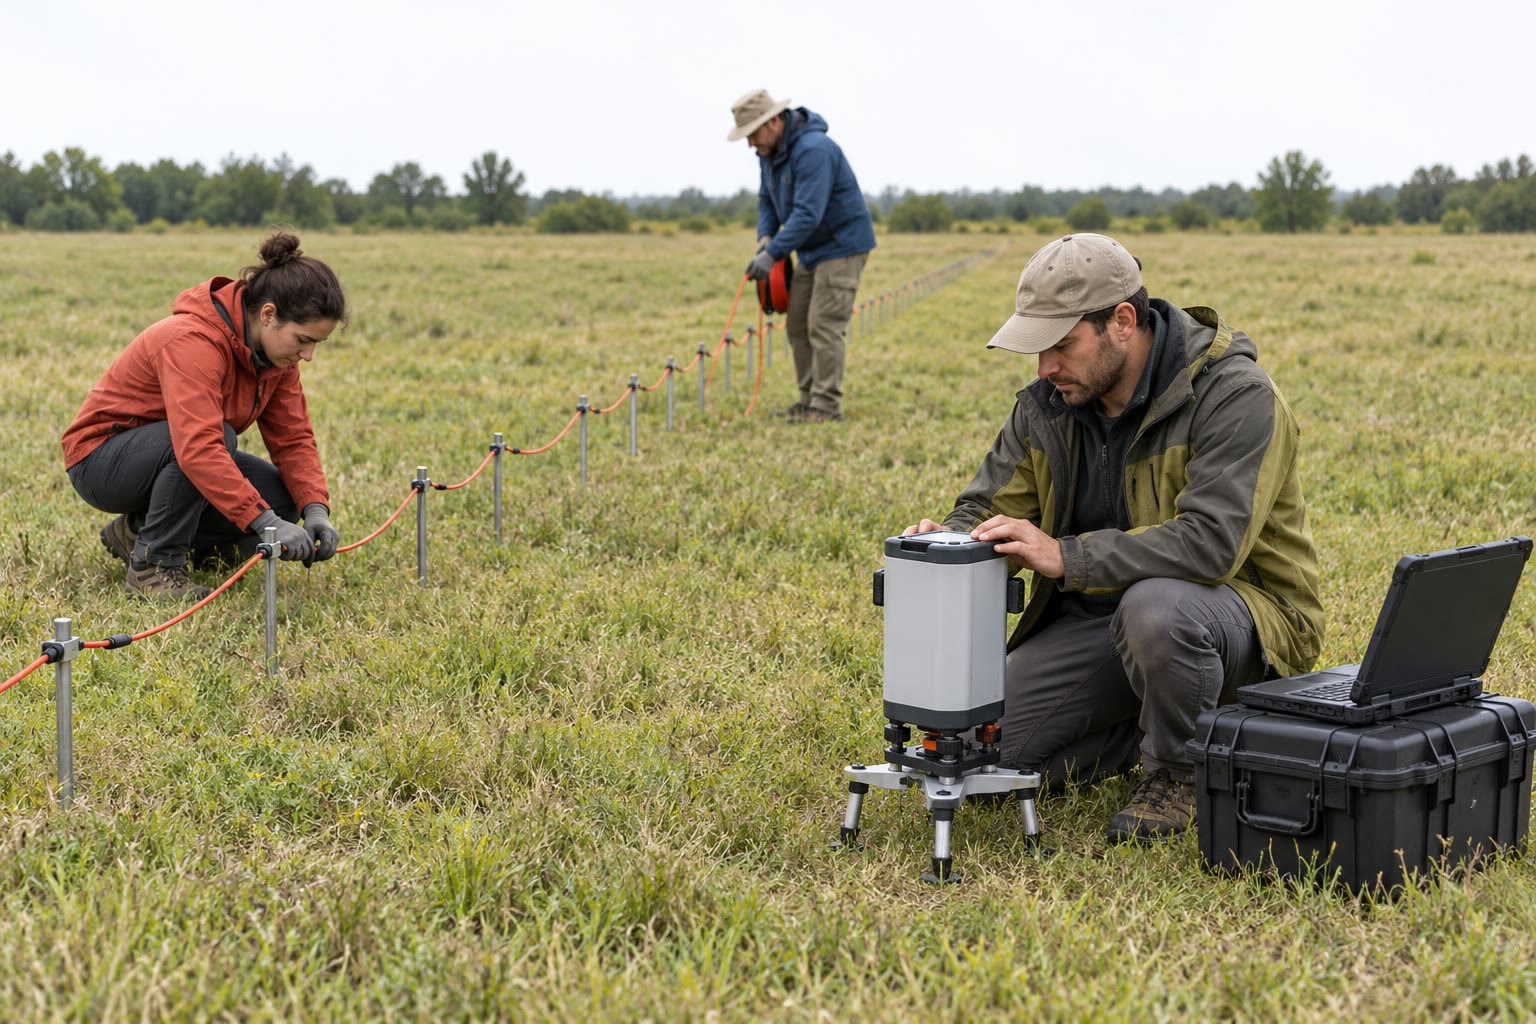
\includegraphics[width=\linewidth]{images/book5/ai/b3-geophysics-crew.jpg}

{\scriptsize Een geofysische ploeg legt een weerstandskabel uit, met een
gravimeter op zijn statief (Door AI gegenereerde illustratie.)}
\end{minipage}
\end{inthefield}

\begin{example}[De Varden-kartering]\label{ex:b3:field-lab-methods-3:varden}
De zwaartekrachtkaart toont een gesloten laagte van ongeveer \qty{-2.3}{\milli\gal}
gecentreerd op het graniet, langgerekt noord--zuid: het lichte graniet
zet zich voort onder de deklaag en is in die richting het langst. De laagte
reikt tot ongeveer \qty{1}{km} van de ontsluiting, zodat het lichaam met de
diepte breder wordt. De halve breedte geeft een eerste diepte voor een equivalente bol;
modellen met een verticale zijkant en een vlakke onderkant laten zien dat een onderkant
tussen één en enkele kilometers diep de piek even goed verklaart, binnen enkele
tienden van een milligal, dus de onderkant blijft onbekend: de niet-eenduidigheid
uit de vorige paragraaf. Op de valleibodem boven het graniet begint de
peiling bij de soortelijke weerstand van droog grind, daalt waar de
stroom het watergezadigde alluvium ingaat en stijgt langs een rechte
lijn met helling één: een geleidende deklaag op een sterk resistieve basis, het
graniet, enkele meters diep. Radar die over dezelfde vloer wordt getrokken toont een
vlakke echo op ongeveer \qty{20}{ns}: de grondwaterspiegel. En de magnetische lijn
over de westelijke flank van de plooi, waar de deklaag dik is en de
sokkelschisten een paar honderd meter diep liggen, registreert een
symmetrisch maximum van ongeveer \qty{20}{nT} dat geen enkele kaart verklaart: een mafische
gang, rijk aan magnetiet, begraven onder de deklaag; de strekking langs de
magnetische meridiaan verklaart waarom de anomalie symmetrisch is. De geofysici
rapporteren hem als een dolerietgang die bij de discordantie werd afgesneden,
en die de deklaag op de kaart verbergt. Het weekendprobleem reduceert de gegevens
van de kartering.
\end{example}
% ledger: gpg:susceptibility, gpg:resistivity, gpg:gpr-table

\section{Oefeningen}

\begin{exercise}[$\star$]\label{exo:b3:field-lab-methods-3:1}
(a)~Welk deel van $g = \qty{9.81}{m.s^{-2}}$ is \qty{0.01}{\milli\gal}?
(b)~Hoeveel moet een gravimeter worden opgetild opdat zijn aflezing verandert
met \qty{0.01}{\milli\gal} door het vrije-luchteffect alleen? (c)~Hoeveel
bedraagt de verandering door het vrije-luchteffect en het Bouguer-effect samen, met de dichtheid
\qty{2670}{kg.m^{-3}}?
\end{exercise}

\begin{exercise}[$\star$]\label{exo:b3:field-lab-methods-3:2}
Een bol met straal \qty{50}{m} en dichtheidscontrast
\qty{+500}{kg.m^{-3}} heeft het middelpunt op \qty{100}{m} diepte. Bereken
de overmassa, de piek van de anomalie en de halve breedte $x_{1/2}$.
\end{exercise}

\begin{exercise}[$\star$]\label{exo:b3:field-lab-methods-3:3}
Een \omterm{def:b3:field-lab-methods-3:resistivity}{Wenner-elektrodeopstelling} met afstand $a = \qty{10}{m}$ injecteert \qty{0.1}{A} en
meet \qty{0.239}{V}. (a)~Bereken de geometriefactor en de
\omterm{def:b3:field-lab-methods-3:resistivity}{schijnbare soortelijke weerstand}. (b)~Toon aan dat een \omterm{def:b3:field-lab-methods-3:resistivity}{Schlumberger-elektrodeopstelling} met $s =
\qty{15}{m}$ en $l = \qty{5}{m}$ dezelfde geometriefactor heeft, en
verklaar waarom.
\end{exercise}

\begin{exercise}[$\star$]\label{exo:b3:field-lab-methods-3:4}
Graniet heeft $\varepsilon_r = 5$. (a)~Bereken de radarsnelheid. (b)~Een
breuk ligt \qty{10}{m} diep: bereken de heen-en-terugtijd van de echo.
(c)~Bereken, met $\sigma = \qty{1}{mS.m^{-1}}$, de huiddiepte en de
bruikbare diepte van ongeveer drie huiddiepten. (d)~Vergelijk met een natte klei met
$\varepsilon_r = 20$ en $\sigma = \qty{10}{mS.m^{-1}}$.
\end{exercise}

\begin{exercise}[$\star\star$]\label{exo:b3:field-lab-methods-3:5}
(a)~Leid de anomalie af van een lange horizontale cilinder met straal $R$ en
dichtheidscontrast $\Delta\rho$, met zijn as op diepte $z$, uit die van een
lijnmassa, en toon aan dat $z = x_{1/2}$. (b)~Een cilinder en een bol
geven dezelfde piek en dezelfde halve breedte $x_{1/2} = \qty{100}{m}$.
Vergelijk hun dieptes. Welke interpretatie geeft het diepere lichaam?
\end{exercise}

\begin{exercise}[$\star\star$]\label{exo:b3:field-lab-methods-3:6}
De Bouguer-anomalie van het Varden-granietmodel, bemonsterd elke
\qty{100}{m} op een kaart van \num{1120} punten die $\qty{3.5}{km}
\times \qty{3.2}{km}$ bestrijken, geeft samen \qty{-438}{\milli\gal}. (a)~Schat met
\cref{prop:b3:field-lab-methods-3:gauss} het massatekort.
(b)~Het massatekort van het model is \qty{1.74e11}{kg}. Welk deel
daarvan vindt de kaart terug, en waar zit de rest?
\end{exercise}

\begin{exercise}[$\star\star$]\label{exo:b3:field-lab-methods-3:7}
(a)~Een dunne gang heeft zijn bovenkant \qty{30}{m} diep. Gebruik de regel van drie
metingen per halve breedte, waarbij de halve breedte de volledige breedte van de
anomalie op de halve piek is. Welke stationsafstand heeft het nodig? (b)~Idem voor
een bovenkant \qty{220}{m} diep. (c)~Waarom kan een enkele kartering niet
zowel een ondiep als een diep lichaam oplossen, tenzij ze voor het ondiepe
is ontworpen?
\end{exercise}

\begin{exercise}[$\star\star$]\label{exo:b3:field-lab-methods-3:8}
Een zandsteen verzadigd met water van \qty{8}{\ohm\metre} heeft een
soortelijke weerstand van \qty{80}{\ohm\metre}. (a)~Bereken met $a = 1$ en $m = 2$
de porositeit. (b)~Herhaal met $m = 1.8$ en $m = 2.2$. Welke
term van de meting bepaalt de onzekerheid van de porositeit?
\end{exercise}

\begin{exercise}[$\star\star$]\label{exo:b3:field-lab-methods-3:9}
(a)~Bereken de eerste drie termen van de tweelaagse reeks
van \cref{prop:b3:field-lab-methods-3:layers} bij $s = 2h_1$ voor $k =
\num{0.5}$ en $k = \num{-0.5}$, en de \omterm{def:b3:field-lab-methods-3:resistivity}{schijnbare soortelijke weerstanden} die
ze opleveren. (b)~Wat zijn de grenswaarden van $\rho_a/\rho_1$ voor $s \ll h_1$ en
$s \gg h_1$? (c)~Welke weerstandsverhoudingen $\rho_2/\rho_1$ horen bij
$k = \pm 0.5$?
\end{exercise}

\begin{exercise}[$\star\star\star$]\label{exo:b3:field-lab-methods-3:10}
(a)~Leid de geometrische factor van de Wenneropstelling af uit
\cref{thm:b3:field-lab-methods-3:point-source}. (b)~Leid die van de
Schlumbergeropstelling af, en toon aan dat $\rho_a \to 2\pi s^2(-\mathrm{d}V/
\mathrm{d}r)/I$ voor $l/s \to 0$. (c)~Hoeveel overschat de benaderde
factor $\pi s^2/(2l)$ de exacte factor bij $l = s/10$?
\end{exercise}

\begin{exercise}[$\star\star\star$]\label{exo:b3:field-lab-methods-3:11}
Een station staat \qty{50}{m} boven de basis. De aflezing is nauwkeurig tot
\qty{0.01}{\milli\gal}, de hoogte tot \qty{5}{cm}; de dichtheid van de
plaat is onzeker met \qty{100}{kg.m^{-3}}, de \omterm{def:b3:field-lab-methods-3:terrain}{terreincorrectie} met
\qty{0.2}{\milli\gal}. (a)~Stel de foutenbegroting op van zijn
Bouguer-anomalie. (b)~Welke term domineert, en welke zou je verbeteren om
een anomalie van \qty{0.1}{\milli\gal} te detecteren? (c)~Wat is het totaal
zonder de terreinterm?
\end{exercise}

\begin{exercise}[$\star\star\star$]\label{exo:b3:field-lab-methods-3:12}
Vijf zwaartekrachtsmetingen over een begraven lichaam, bij $x = -600$, $-300$, $0$,
$300$ en \qty{600}{m}, zijn \num{-0.69}, \num{-2.17}, \num{-4.16},
\num{-2.10} en \qty{-0.73}{\milli\gal}, elk met $\sigma =
\qty{0.03}{\milli\gal}$. (a)~Kies voor bolmodellen gecentreerd onder $x = 0$ op
dieptes van \num{300}, \num{400} en \qty{500}{m}, kies de massa die bij de
centrale aflezing past, en bereken de \omterm{def:b3:field-lab-methods-3:inversion-practice}{misfit} $\chi^2$ van elk. (b)~Welk
model past binnen de fouten bij de data? (c)~Zou een lichaam van een andere
vorm even goed passen? Wat zou dat beslissen?
\end{exercise}

\section{Probleem: De verborgen lichamen van de Varden Hills}

\begin{problem}[{Weekendprobleem --- de Varden-meting reduceren}]
\label{pb:b3:field-lab-methods-3:1}
Gebruik $G = \qty{6.674e-11}{m^3.kg^{-1}.s^{-2}}$, de vrije-luchtgradiënt
\qty{0.3086}{\milli\gal.m^{-1}} en de Bouguer-factor
\qty{0.1119}{\milli\gal.m^{-1}} (dichtheid \qty{2670}{kg.m^{-3}}).

\medskip\noindent\textbf{Deel I --- Een zwaartekrachtlus.} Een lus op het
zwaartekrachtprofiel geeft (aflezingen in milligal na kalibratie, hoogten
in meter, tijden in uren na 09:00):
\begin{center}
\small
\begin{tabular}{lccccc}
\hline
station & basis & \qty{3.0}{km} & \qty{3.5}{km} & \qty{4.0}{km} & basis \\
\hline
tijd & 0 & 0.5 & 0.9 & 1.3 & 2.0 \\
hoogte & 176.1 & 149.0 & 145.5 & 158.0 & 176.1 \\
aflezing & 2846.512 & 2851.075 & 2850.497 & 2849.392 & 2846.708 \\
\hline
\end{tabular}
\end{center}
\begin{enumerate}
\item Bereken de driftsnelheid van de lus.
\item Corrigeer de drie stationsaflezingen voor de drift en druk ze
  uit ten opzichte van de basis.
\item Pas de vrije-lucht- en Bouguer-correcties toe voor de
  hoogteverschillen, en geef de Bouguer-anomalie van elk station ten opzichte van
  de basis.
\item De drift van het instrument alleen bedroeg \qty{0.040}{\milli\gal.h^{-1}}. Wat veroorzaakte
  de rest van de verandering bij de basis, en waarom kon die met de
  drift worden verwijderd?
\item Het model waaruit de aflezingen komen, geeft de drie anomalieën
  ten opzichte van de basis als \num{-0.825}, \num{-2.131} en
  \qty{-0.825}{\milli\gal}. Bereken de fouten van de reductie. De
  hoogten in de tabel zijn afgerond op \qty{0.1}{m}: welke fout kan deze
  afronding introduceren, en verklaart die de fouten?
\item Welke hoognauwkeurigheid houdt de gereduceerde anomalie binnen
  \qty{0.01}{\milli\gal}? Waarom vragen handleidingen voor metingen om
  \qty{3.3}{cm}, een strengere eis?
\end{enumerate}

\medskip\noindent\textbf{Deel II --- De anomalie van het graniet.} Langs
het profiel heeft de anomalie haar minimum, \qty{-2.293}{\milli\gal}, bij
$x = \qty{3.50}{km}$, en bereikt ze de helft van die waarde bij $x = 3.048$ en
\qty{3.952}{km}. Het granietmodel heeft een dichtheidscontrast van
\qty{-130}{kg.m^{-3}}, en het maaiveld in het midden ligt \qty{145.5}{m}
boven zeeniveau.
\begin{enumerate}[resume]
\item Bereken de halve breedte $x_{1/2}$ en de diepte van het middelpunt van
  de equivalente bol.
\item Bereken het massatekort van die bol en de straal ervan voor het
  dichtheidscontrast van het graniet. Wat valt op aan het resultaat?
\item Het massamiddelpunt van het model ligt \qty{864}{m} onder het maaiveld en
  het massatekort bedraagt \qty{1.74e11}{kg}. Waarom geeft de halve-breedteregel een
  ondieper en lichter lichaam?
\item Een verticale cilinder met hetzelfde oppervlak als het graniet op de
  discordantie heeft een straal van \qty{461}{m}. Bereken de anomalie op de as
  voor een bovenkant aan het maaiveld en een onderkant op \qty{1645}{m} diepte, en voor
  een onbeperkte diepte.
\item Zoek, door te proberen of door op te lossen, de diepte van de onderkant waarvoor
  deze cilinder de waargenomen \qty{-2.29}{\milli\gal} geeft.
\item Bereken de anomalie van de cilinder met de bovenkant \qty{6}{m} diep
  (onderkant \qty{1645}{m}). Kan de zwaartekracht onderscheiden of het graniet
  onder het alluvium tot aan het oppervlak reikt?
\end{enumerate}

\medskip\noindent\textbf{Deel III --- De dalbodem.} De Schlumbergersondering op de bodem
boven het graniet geeft (halve afstand $s$ in
meter, $\rho_a$ in \unit{\ohm\metre}):
\begin{center}
\small
\begin{tabular}{lcccccccc}
\hline
$s$ & 1 & 2 & 4 & 6 & 10 & 20 & 30 & 40 \\
$\rho_a$ & 577 & 526 & 387 & 350 & 449 & 821 & 1309 & 1684 \\
\hline
\end{tabular}
\end{center}
Op een radarprofiel langs dezelfde bodem geeft een pijp een hyperbool met
zijn top bij \qty{10.7}{ns} en een looptijd van \qty{17.1}{ns} op \qty{1}{m}
opzij; een vlakke echo komt aan bij \qty{20.0}{ns}.
\begin{enumerate}[resume]
\item Bij $s = \qty{20}{m}$ was MN \qty{2}{m} lang en de stroom
  \qty{50}{mA}. Bereken de geometrische factor en de gemeten spanning.
\item Bereken de radarsnelheid, de relatieve permittiviteit van het
  alluvium en de diepte van de pijp.
\item De vlakke echo is de grondwaterspiegel. Hoe diep ligt die?
\item Schat de geleidbaarheid $S$ van het alluvium uit de aflezingen bij
  20, 30 en \qty{40}{m}.
\item Het droge alluvium heeft \qty{600}{\ohm\metre}, en het verzadigde
  alluvium \qty{222}{\ohm\metre}. Bereken de dikte van het verzadigde
  alluvium en de diepte van de bovenkant van het graniet. Is de schatting hoog
  of laag, en waarom?
\item Het grondwater heeft \qty{20}{\ohm\metre}. Bereken de porositeit van
  het alluvium met de \omterm{prop:b3:field-lab-methods-3:archie}{wet van Archie} bij $m = 2$, en het bereik van $m$
  tussen \num{1.3} en \num{2.8}.
\end{enumerate}

\medskip\noindent\textbf{Deel IV --- De magnetische lijn.} De lijn loopt
vanaf $x = \qty{1.70}{km}$ naar het oosten, met één station per \qty{50}{m} en
elke twee minuten; het basisstation registreerde op dezelfde minuten. De
aflezingen, min \qty{48000}{nT}, zijn:
\begin{center}
\small
\setlength{\tabcolsep}{3.5pt}
\begin{tabular}{lccccccccccc}
\hline
$x$ (km) & 1.70 & 1.75 & 1.80 & 1.85 & 1.90 & 1.95 & 2.00 & 2.05 & 2.10 & 2.15 & 2.20 \\
lijn & 3.4 & 4.8 & 6.3 & 8.1 & 10.3 & 12.8 & 15.8 & 19.2 & 22.9 & 26.2 & 28.0 \\
basis & 0.0 & 0.7 & 1.5 & 2.2 & 2.9 & 3.6 & 4.3 & 5.0 & 5.7 & 6.4 & 7.0 \\
\hline
$x$ (km) & 2.25 & 2.30 & 2.35 & 2.40 & 2.45 & 2.50 & 2.55 & 2.60 & 2.65 & 2.70 & \\
lijn & 27.7 & 25.8 & 23.3 & 20.9 & 19.0 & 17.6 & 16.6 & 15.9 & 15.5 & 15.2 & \\
basis & 7.6 & 8.2 & 8.8 & 9.4 & 9.9 & 10.4 & 10.9 & 11.3 & 11.7 & 12.1 & \\
\hline
\end{tabular}
\end{center}
Het hoofdveld bedraagt \qty{48000}{nT}, met een inclinatie van \ang{65}.
\begin{enumerate}[resume]
\item Pas de \omterm{def:b3:field-lab-methods-3:magnetic}{dagelijkse correctie} toe en geef de gecorrigeerde anomalie bij
  elk station.
\item Toon aan dat de anomalie zonder de correctie aan de oostkant nooit tot de
  helft van haar piek daalt.
\item Bepaal de piek en de twee punten waar de gecorrigeerde anomalie de
  helft van de piek bereikt, door lineaire interpolatie, en bereken de halfwaardebreedte.
\item De anomalie is symmetrisch. Wat zegt dat over de strekking van
  het lichaam, en welk soort lichaam veronderstelt de halfwaardebreedteregel?
\item Bereken het product $\kappa t$ van susceptibiliteit en dikte.
  Als de gang uit doleriet bestaat met een susceptibiliteit van \num{0.03}, hoe dik is
  de gang?
\item Waren de stations dicht genoeg bij elkaar?
\item Bepaal de diepte tot de bovenkant van de verborgen gang onder het maaiveld, op
  de dichtstbijzijnde tien meter, en vergelijk die met de diepte van de
  discordantie in het geologische model van het gebied, \qty{222}{m} op dit
  punt.
\end{enumerate}
\end{problem}
% ledger: gpg:grav-survey, gpg:mag-field, keys:archie
